\documentclass[a4paper,11pt]{article}
\usepackage{amsmath,latexsym}
\usepackage{geometry}
\usepackage{graphicx}
\geometry{left=2.5cm,right=2.5cm,top=2.5cm,bottom=2.5cm}
\usepackage{caption,subcaption}
\usepackage{listings}
\lstset{language=Matlab}
\lstset{breaklines}
\lstset{extendedchars=false}
\usepackage{xcolor}
\usepackage{graphicx}
\usepackage[round]{natbib}
\usepackage{indentfirst}
\setlength{\parindent}{2em}

\begin{document}
\title{\Large{PP plot against Generalized Extreme Value Distribution}}
\date{July 18th, 2016}
\maketitle
\begin{flushleft}

Project members:\\

\hspace{1.5cm} Jia Huang 27720151153586\hspace{1.5cm}    Shaoying Yang 27720151153593\\
 \hspace{1.5cm} Huijian Sun 27720151153591 \hspace{1.05cm}   Yaxi Li 27720151153587\\



\section{Introduction}

PP plot of tail values of daily log-returns of portfolio against Generalized Extreme Value Distribution with a global parameter $\gamma$ estimated with the block maxima method.\\

\section{Data source}

\begin{enumerate}
\item Data websites: \begin{itemize}
\item	http://finance.yahoo.com/quote/BAYN.DE/history\\
\item    http://finance.yahoo.com/quote/BMW.DE/history\\
\item   http://finance.yahoo.com/quote/SIE.DE/history\\
\end{itemize}
\item Data range: all the trading days from $2000-01-01$ to $2016-07-11$, daily data.\\

\item Data files: $close.csv$\\

\end{enumerate}


\section{Procedure}
\begin{enumerate}
\item Construct a portfolio: $p=Bayer+Bmw+Siemens$.\\

\item Calculate the parameters of the portfolio by using Block Maxima Model.\\
 \begin{enumerate}
	
  \item Decompose negative returns $\{X_t\}_{t=1}^T$ into $k$ non-overlapping sets.\\

  \item Define $\{Z_j\}_{j=1}^k$ where $Z_j=max\{X_{(j-1)n+1},...,X_{jn}\}$.\\

 \item For $\{Z_j\}_{j=1}^k$, fit generalized extreme value distribution $G_{\gamma}(\frac{x-\mu}{\sigma})$.\\

 \item Get the shape parameter $\gamma$, the location parameter $\mu$ and the scale parameter $\sigma$.\\
  T denotes the number of observations.\\
 \end{enumerate}
 
\item Plot the PP plot.\\
\begin{enumerate}
\item Use static windows of size w = 214 scrolling in time t for VaR estimation $\left \{ X_t \right \}_{t=s-w+1}^{s}$ for $s = w,\cdots ,T$ .\\

\item Plot the PP plot for static windows of size w.\\
\end{enumerate}

\end{enumerate}
\section{Plots}
The PP plot against the Generalized Extreme Value Distribution is shown in the following figure\\

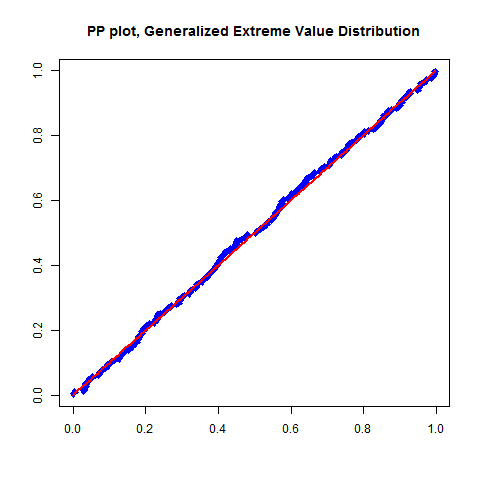
\includegraphics{SFMTailGEV}

\section{R Code}

\lstset{                        %Settings for listings package.
  language=[ANSI]{C},
  basicstyle=\footnotesize,
  breakatwhitespace=false,
  breaklines=true,
  captionpos=b,
  commentstyle=\color{olive},
  directivestyle=\color{blue},
  extendedchars=false,
  % frame=single,%shadowbox
  framerule=0pt,
  keywordstyle=\color{blue}\bfseries,
  morekeywords={*,define,*,include...},
  numbersep=5pt,
  rulesepcolor=\color{red!20!green!20!blue!20},
  showspaces=false,
  showstringspaces=false,
  showtabs=false,
  stepnumber=2,
  stringstyle=\color{purple},
  tabsize=4,
  title=\lstname
}

{\linespread{1.5}\selectfont
\begin{lstlisting}
# clear variables and close windows
rm(list = ls(all = TRUE))
graphics.off()
# install and load packages
libraries = c("fExtremes")
lapply(libraries, function(x) if (!(x %in% installed.packages())) {install.packages(x)})
lapply(libraries, library, quietly = TRUE, character.only = TRUE)
# load data
dat <- read.table(file="close.csv",header = TRUE,stringsAsFactors = FALSE,sep= ",")
# Portfolio
p = dat$Bayer.Close.Price + dat$BMW.Close.Price + dat$Siemens.Close.Price
l = length(p)  # length of portfolio
loss  = log(p[1:(l - 1)]/p[2:l])  # negative log-returns
# Determine the Block Maxima data
T = length(loss)
n = 20
k = T/n
z = matrix(, , )
for (j in 1:k) {
        d = loss[((j - 1) * n + 1):(j * n)]
        z[j] = max(d)
}
w = sort(z)
# Fit the Generalized Extreme Value Distribution
GEV = gevFit(w, type = "mle")
# shape parameter
gama = attr(GEV, "fit")$par.ests[1]
gama
# location parameter
mu = attr(GEV, "fit")$par.ests[2]
# scale parameter
sigma = attr(GEV, "fit")$par.ests[3]
t = (1:k)/(k + 1)
y = pgev(w, xi = gama, mu = mu, beta = sigma)
# Plot the PP plot
dev.new()
png("SFMTailGEV.png")
plot(y, t, col = "blue", pch = 23, bg = "blue", xlab = c(""), ylab = c(""))
lines(y, y, type = "l", col = "red", lwd = 2)
title("PP plot, Generalized Extreme Value Distribution")
\end{lstlisting}
}
\end{flushleft}
	
\end{document}



